\documentclass{standalone}
\usepackage{tikz}
\usepackage{ctex,siunitx}
\setCJKmainfont{Noto Serif CJK SC}
\usepackage{tkz-euclide}
\usepackage{amsmath}
\usetikzlibrary{patterns, calc,3d}
\usetikzlibrary {decorations.pathmorphing,decorations.pathreplacing,decorations.shapes}
\begin{document}
\small
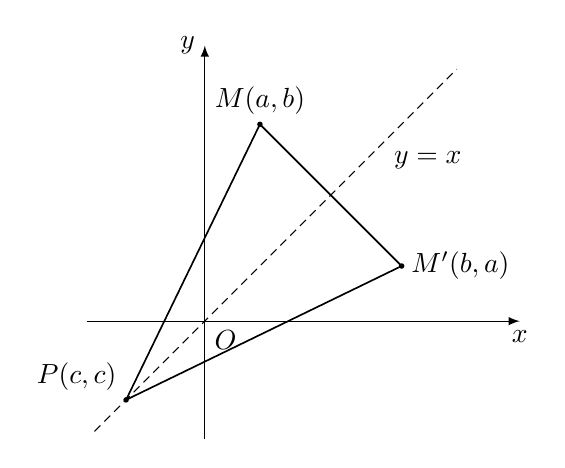
\begin{tikzpicture}[>=latex,scale=1.0]
  \draw[->](-1.5,0)--(4,0)node[below]{$x$};
  \draw[->](0,-1.5)--(0,3.5)node[left]{$y$};
  \node at (0,0)[below right]{$O$};
  \draw[densely dashed](-1.4,-1.4)--(3.2,3.2)node[pos=0.8,below right]{$y=x$};
  \coordinate (P) at (-1,-1);\node at (P)[above left]{$P(c,c)$};
  \coordinate (M) at (0.7,2.5);\node at (M)[above]{$M(a,b)$};
  \coordinate (M') at (2.5,0.7);\node at (M')[right]{$M'(b,a)$};
  \foreach \x in {P,M,M'} {\fill(\x)circle(1pt);}
  \draw[semithick](P)--(M)(P)--(M')(M)--(M');
\end{tikzpicture}
\end{document}